% This file is generated by the MATLAB m-file laprint.m. It can be included
% into LaTeX documents using the packages graphicx, color and psfrag.
% It is accompanied by a postscript file. A sample LaTeX file is:
%    \documentclass{article}\usepackage{graphicx,color,psfrag}
%    \begin{document}% This file is generated by the MATLAB m-file laprint.m. It can be included
% into LaTeX documents using the packages graphicx, color and psfrag.
% It is accompanied by a postscript file. A sample LaTeX file is:
%    \documentclass{article}\usepackage{graphicx,color,psfrag}
%    \begin{document}% This file is generated by the MATLAB m-file laprint.m. It can be included
% into LaTeX documents using the packages graphicx, color and psfrag.
% It is accompanied by a postscript file. A sample LaTeX file is:
%    \documentclass{article}\usepackage{graphicx,color,psfrag}
%    \begin{document}% This file is generated by the MATLAB m-file laprint.m. It can be included
% into LaTeX documents using the packages graphicx, color and psfrag.
% It is accompanied by a postscript file. A sample LaTeX file is:
%    \documentclass{article}\usepackage{graphicx,color,psfrag}
%    \begin{document}\input{f1app}\end{document}
% See http://www.mathworks.de/matlabcentral/fileexchange/loadFile.do?objectId=4638
% for recent versions of laprint.m.
%
% created by:           LaPrint version 3.15 (29.4.2004)
% created on:           04-Feb-2008 11:02:53
% eps bounding box:     15 cm x 11.25 cm
% comment:              
%
\begin{psfrags}%
\psfragscanon%
%
% text strings:
\psfrag{s05}[t][t]{\setlength{\tabcolsep}{0pt}\begin{tabular}{c}$x_1$\end{tabular}}%
\psfrag{s06}[b][b]{\setlength{\tabcolsep}{0pt}\begin{tabular}{c}$f_1(x_1)$\end{tabular}}%
\psfrag{s10}[l][l]{$\hat f_1(x_1)$}%
\psfrag{s11}[l][l]{$f_1(x_1)$}%
\psfrag{s12}[l][l]{$\hat f_1(x_1)$}%
%
% xticklabels:
\psfrag{x01}[t][t]{-3.1416}%
\psfrag{x02}[t][t]{-0.8976}%
\psfrag{x03}[t][t]{0.8976}%
\psfrag{x04}[t][t]{3.1416}%
%
% yticklabels:
\psfrag{v01}[r][r]{-1}%
\psfrag{v02}[r][r]{-0.8}%
\psfrag{v03}[r][r]{-0.6}%
\psfrag{v04}[r][r]{-0.4}%
\psfrag{v05}[r][r]{-0.2}%
\psfrag{v06}[r][r]{0}%
\psfrag{v07}[r][r]{0.2}%
\psfrag{v08}[r][r]{0.4}%
\psfrag{v09}[r][r]{0.6}%
\psfrag{v10}[r][r]{0.8}%
\psfrag{v11}[r][r]{1}%
%
% Figure:
\resizebox{12cm}{!}{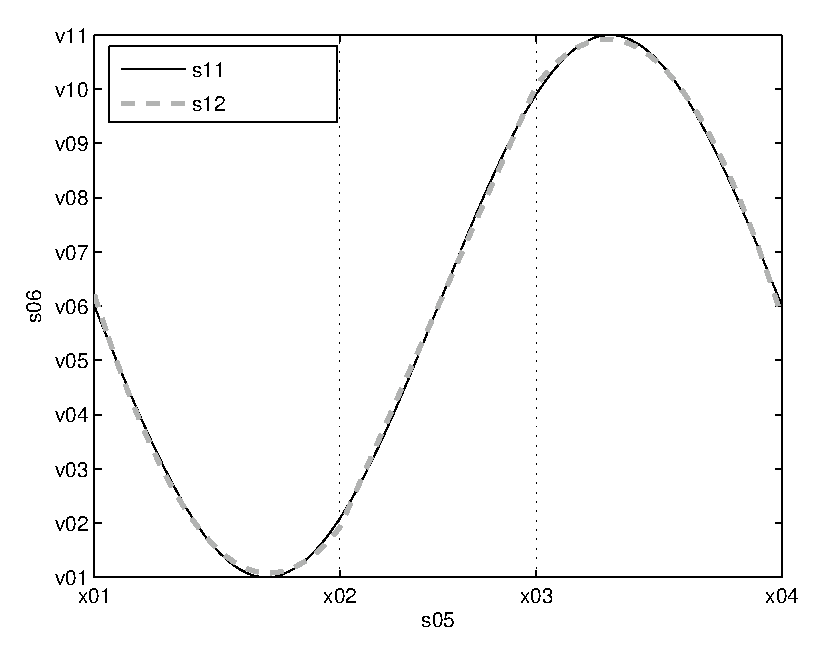
\includegraphics{images/f1app.eps}}%
\end{psfrags}%
%
% End f1app.tex
\end{document}
% See http://www.mathworks.de/matlabcentral/fileexchange/loadFile.do?objectId=4638
% for recent versions of laprint.m.
%
% created by:           LaPrint version 3.15 (29.4.2004)
% created on:           04-Feb-2008 11:02:53
% eps bounding box:     15 cm x 11.25 cm
% comment:              
%
\begin{psfrags}%
\psfragscanon%
%
% text strings:
\psfrag{s05}[t][t]{\setlength{\tabcolsep}{0pt}\begin{tabular}{c}$x_1$\end{tabular}}%
\psfrag{s06}[b][b]{\setlength{\tabcolsep}{0pt}\begin{tabular}{c}$f_1(x_1)$\end{tabular}}%
\psfrag{s10}[l][l]{$\hat f_1(x_1)$}%
\psfrag{s11}[l][l]{$f_1(x_1)$}%
\psfrag{s12}[l][l]{$\hat f_1(x_1)$}%
%
% xticklabels:
\psfrag{x01}[t][t]{-3.1416}%
\psfrag{x02}[t][t]{-0.8976}%
\psfrag{x03}[t][t]{0.8976}%
\psfrag{x04}[t][t]{3.1416}%
%
% yticklabels:
\psfrag{v01}[r][r]{-1}%
\psfrag{v02}[r][r]{-0.8}%
\psfrag{v03}[r][r]{-0.6}%
\psfrag{v04}[r][r]{-0.4}%
\psfrag{v05}[r][r]{-0.2}%
\psfrag{v06}[r][r]{0}%
\psfrag{v07}[r][r]{0.2}%
\psfrag{v08}[r][r]{0.4}%
\psfrag{v09}[r][r]{0.6}%
\psfrag{v10}[r][r]{0.8}%
\psfrag{v11}[r][r]{1}%
%
% Figure:
\resizebox{12cm}{!}{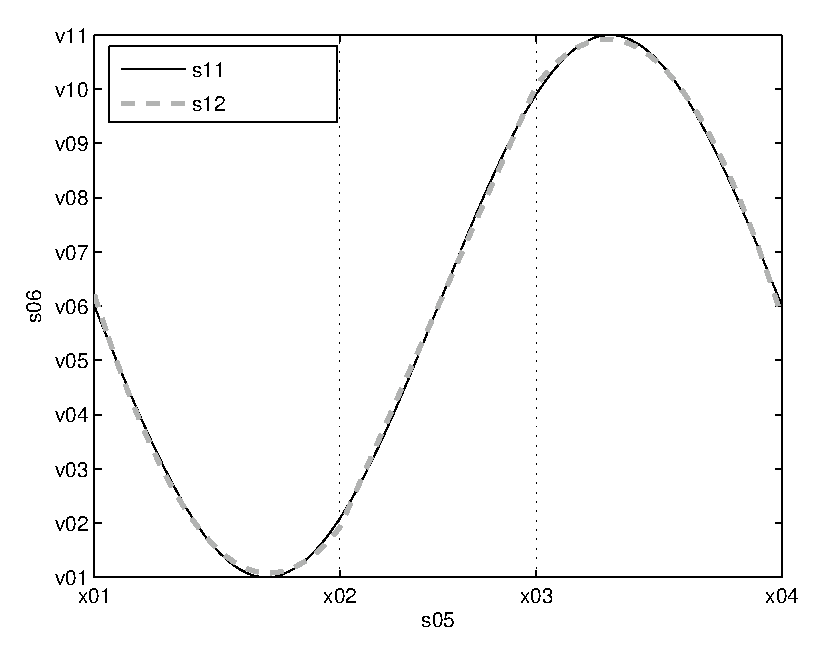
\includegraphics{images/f1app.eps}}%
\end{psfrags}%
%
% End f1app.tex
\end{document}
% See http://www.mathworks.de/matlabcentral/fileexchange/loadFile.do?objectId=4638
% for recent versions of laprint.m.
%
% created by:           LaPrint version 3.15 (29.4.2004)
% created on:           04-Feb-2008 11:02:53
% eps bounding box:     15 cm x 11.25 cm
% comment:              
%
\begin{psfrags}%
\psfragscanon%
%
% text strings:
\psfrag{s05}[t][t]{\setlength{\tabcolsep}{0pt}\begin{tabular}{c}$x_1$\end{tabular}}%
\psfrag{s06}[b][b]{\setlength{\tabcolsep}{0pt}\begin{tabular}{c}$f_1(x_1)$\end{tabular}}%
\psfrag{s10}[l][l]{$\hat f_1(x_1)$}%
\psfrag{s11}[l][l]{$f_1(x_1)$}%
\psfrag{s12}[l][l]{$\hat f_1(x_1)$}%
%
% xticklabels:
\psfrag{x01}[t][t]{-3.1416}%
\psfrag{x02}[t][t]{-0.8976}%
\psfrag{x03}[t][t]{0.8976}%
\psfrag{x04}[t][t]{3.1416}%
%
% yticklabels:
\psfrag{v01}[r][r]{-1}%
\psfrag{v02}[r][r]{-0.8}%
\psfrag{v03}[r][r]{-0.6}%
\psfrag{v04}[r][r]{-0.4}%
\psfrag{v05}[r][r]{-0.2}%
\psfrag{v06}[r][r]{0}%
\psfrag{v07}[r][r]{0.2}%
\psfrag{v08}[r][r]{0.4}%
\psfrag{v09}[r][r]{0.6}%
\psfrag{v10}[r][r]{0.8}%
\psfrag{v11}[r][r]{1}%
%
% Figure:
\resizebox{12cm}{!}{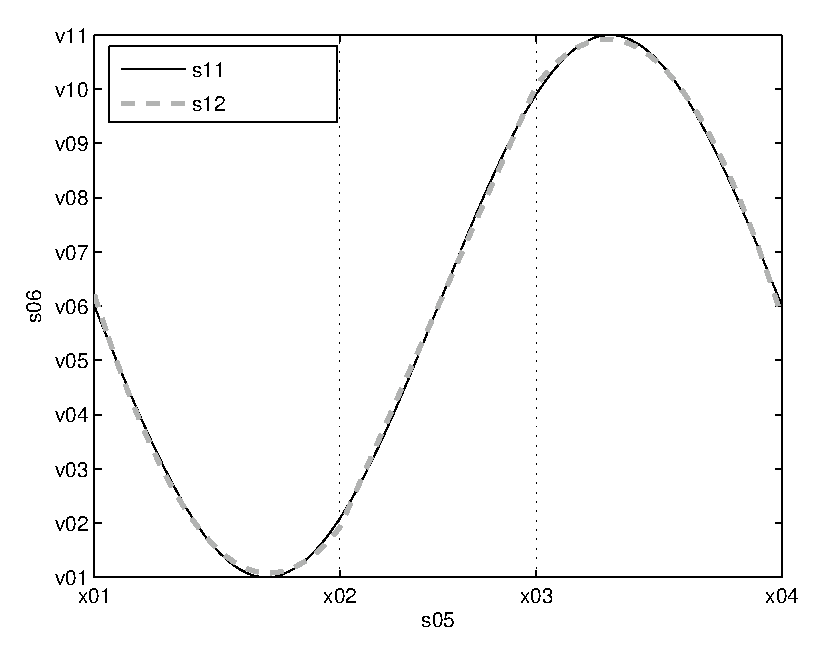
\includegraphics{images/f1app.eps}}%
\end{psfrags}%
%
% End f1app.tex
\end{document}
% See http://www.mathworks.de/matlabcentral/fileexchange/loadFile.do?objectId=4638
% for recent versions of laprint.m.
%
% created by:           LaPrint version 3.15 (29.4.2004)
% created on:           04-Feb-2008 11:02:53
% eps bounding box:     15 cm x 11.25 cm
% comment:              
%
\begin{psfrags}%
\psfragscanon%
%
% text strings:
\psfrag{s05}[t][t]{\setlength{\tabcolsep}{0pt}\begin{tabular}{c}$x_1$\end{tabular}}%
\psfrag{s06}[b][b]{\setlength{\tabcolsep}{0pt}\begin{tabular}{c}$f_1(x_1)$\end{tabular}}%
\psfrag{s10}[l][l]{$\hat f_1(x_1)$}%
\psfrag{s11}[l][l]{$f_1(x_1)$}%
\psfrag{s12}[l][l]{$\hat f_1(x_1)$}%
%
% xticklabels:
\psfrag{x01}[t][t]{-3.1416}%
\psfrag{x02}[t][t]{-0.8976}%
\psfrag{x03}[t][t]{0.8976}%
\psfrag{x04}[t][t]{3.1416}%
%
% yticklabels:
\psfrag{v01}[r][r]{-1}%
\psfrag{v02}[r][r]{-0.8}%
\psfrag{v03}[r][r]{-0.6}%
\psfrag{v04}[r][r]{-0.4}%
\psfrag{v05}[r][r]{-0.2}%
\psfrag{v06}[r][r]{0}%
\psfrag{v07}[r][r]{0.2}%
\psfrag{v08}[r][r]{0.4}%
\psfrag{v09}[r][r]{0.6}%
\psfrag{v10}[r][r]{0.8}%
\psfrag{v11}[r][r]{1}%
%
% Figure:
\resizebox{12cm}{!}{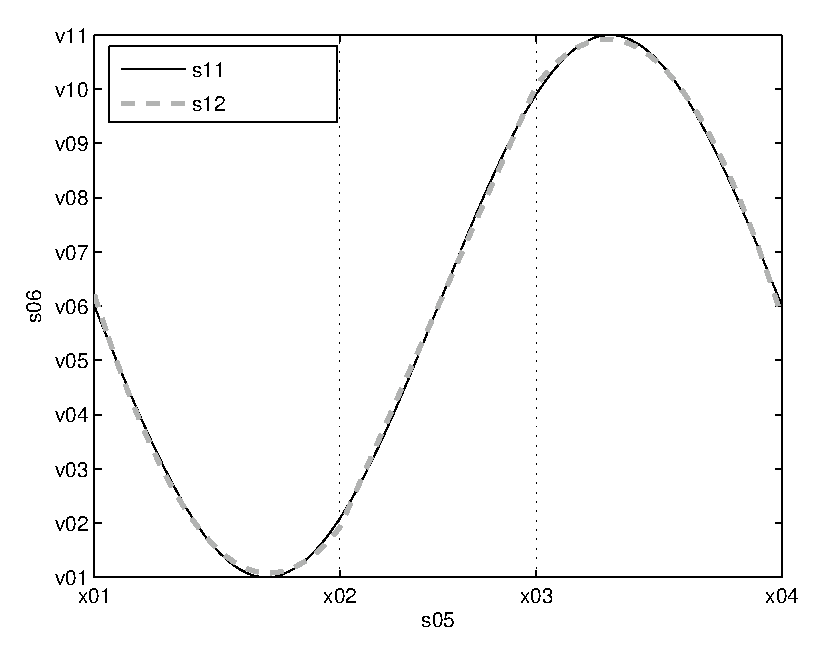
\includegraphics{images/f1app.eps}}%
\end{psfrags}%
%
% End f1app.tex
